\documentclass[fleqn,10pt]{wlscirep}
\usepackage[utf8]{inputenc}
\usepackage[T1]{fontenc}
\usepackage{times}
\usepackage{epsfig}
\usepackage{graphicx}
\usepackage{amsmath}
\usepackage{amssymb}
\usepackage{soul}
\usepackage{xcolor}
\usepackage{mathbbol}
\usepackage{multicol}
\usepackage[numbers,sort&compress]{natbib}

\newcommand{\NCMRGBR}{29,103\,}
\newcommand{\NCALLS}{801,526\,} % Number of genotyped SNPs 
\newcommand{\MAFTHR}{1\% } % MAF threshold (in percentage)
\newcommand{\NIMP}{more than 90 million\,} % number of imputed variants with MAF > threshold
\newcommand{\HWEPVAL}{$10^{-6}$} % Hardy-Weinberg equilibrium p-value threshold
\newcommand{\LVNP}{2,677} % number of points in the LV mesh
\newcommand{\NGWASHITS}{10}

% ANONYMISED VERSION 
% \newcommand{\ACCESSIONNUMBER}{---}

\newcommand{\ACCESSIONNUMBER}{11350}

\def\code#1{\texttt{#1}} 

\usepackage{graphicx}

\begin{document}
\title{Unsupervised deep learning helps disentangle the genetic basis of cardiac morphology: Supplementary Material}

\author[1,2,*]{Rodrigo Bonazzola}
\author[1,2]{Andres Diaz-Pinto}
\author[1,2]{Avan Suinesiaputra}
\author[1,2]{Rahman Attar}
\author[1,2]{Nishant Ravikumar}
\author[2]{Eylem Levelt}
\author[2]{Sven Plein}
\author[3]{Enzo Ferrante}
\author[4]{Tanveer Syeda-Mahmood}
\author[1,2,5]{Alejandro F Frangi}
\affil[1]{Centre for Computational Imaging and Simulation Technologies in Biomedicine (CISTIB), School of Computing and School of Medicine, University of Leeds, Leeds, UK}
\affil[2]{Leeds Institute of Cardiovascular and Metabolic Medicine, School of Medicine, University of Leeds, Leeds, UK}
\affil[3]{Research Institute for Signals, Systems and Computational Intelligence, sinc(i), FICH-UNL / CONICET, Santa Fe, Argentina}
\affil[4]{IBM Almaden Research Center, San Jose, USA
}
\affil[5]{Medical Imaging Research Center (MIRC), University Hospital Gasthuisberg. Cardiovascular Sciences and Electrical Engineering Departments, KU Leuven, Leuven, Belgium}

\affil[*]{scrb@leeds.ac.uk}

\maketitle              % typeset the header of the contribution

\section{Code and data}
The code used to produce the results of this paper has been provided in two folders:  \code{CoMA} and \code{GWAS\_pipeline}. The first one contains the code for executing the CoMA experiments, the other contains the code for performing GWAS and generating the associated plots.

The genetic and imaging data used for this work has been downloaded from the UK Biobank (UKB). Since this is protected data for which access must be granted by the UKB, it has not been included in this submission.

% \newline
\textbf{Morphological interpretation of the latent basis.} An interpretation of the impact of each of the components of the latent basis on LV morphology was achieved by varying the components of the latent space one at a time and generating the associated synthetic shapes by means of the trained decoder. % heat map showing the deviations from the mean shape. 
In the main text of this paper, only those components that yielded Bonferroni-significant SNP associations are shown, along with the corresponding Manhattan plots. The rest of them are included in this supplementary material.

\section{Dimensionality reduction and GWAS}

Different dimensions of the latent space $n_z$ and weights $w_{\textrm{KL}}$ were studied, the aim being to achieve a compromise between reconstruction error and interpretability (and hence heritability) of the components.

Figure \ref{fig:pca_vs_coma} shows a comparison of the reconstruction error obtained through PCA and CoMA, as a function of the number of the components $n_z$ of the latent space. CoMA and PCA yield comparable reconstruction errors, with CoMA outperforming the latter slightly. No significant difference was found between non-variational and variational CoMA.
%whereas increasing $w_\text{KL}$ leads to worse quality of the reconstructions, as expected. 
Also, adding the $D_\textrm{KL}$ regularisation term leads to the expected statistical properties of the latent representation of the shapes (independence and isotropy), as can be seen in the supplementary material.

\begin{figure}[ht!]
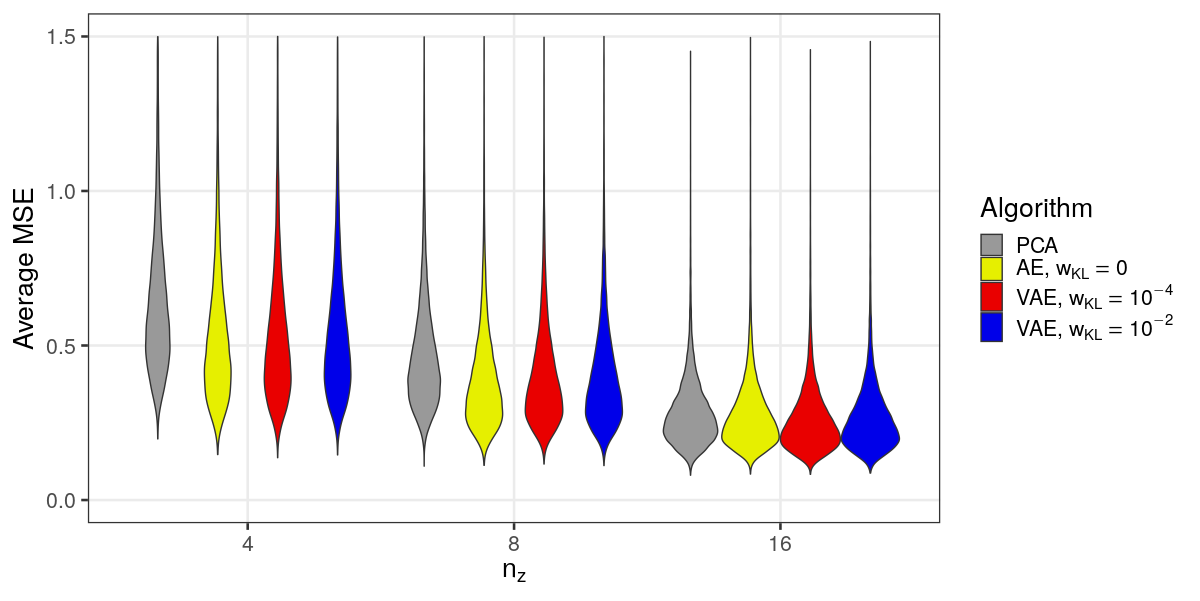
\includegraphics[width=\linewidth]{figs/performance.png}
\caption{Distribution of reconstruction errors (measured as the MSE averaged across the vertices of the mesh) for models trained with different number of components in the latent space, using PCA and CoMA. As a reference, given the vertex-wise normalization that is performed on the meshes, if the real and reconstructed shapes are totally independent the expected value of MSE would be around 2, whereas if we reconstruct the mean shape it would be around 1.}
\label{fig:pca_vs_coma}
\end{figure}

\subsection{Implementation details}
For the autoencoder, we ran a grid optimisation scheme for meta-parameter selection, both for the architecture and the learning process. For each number of components $n_z$ and regularisation weight $w_\textrm{KL}$, the execution that presented the minimum mean squared error (MSE) within the validation set was chosen.
The autoencoder architecture is explained in table \ref{table:AE_arch}. After each convolutional layer, a ReLU activation function was applied. The number of samples used for training was 5,000, whereas the validation set contained 1,000 individuals. The Adam optimiser was used to find optimal network parameters, by minimising the MSE reconstruction loss.

\begin{table}
\begin{center}
\begin{tabular}{|c|c|c|}
\hline
          & \textbf{Input} & \textbf{Output} \\ \hline
ChebConv  & $2677\times 3$ &  $2677\times 16$ \\ \hline
DS        & $2677\times 16$ & $670\times 16$ \\ \hline
ChebConv  & $670\times 16$ & $670\times 16$ \\ \hline
DS        & $670\times 16$ & $168\times 16$ \\ \hline
ChebConv  & $168\times 16$ & $168\times 16$ \\ \hline
DS        & $168\times 16$ & $56\times 16$\\ \hline
ChebConv  & $56\times 16$ &  $56\times 32$\\ \hline
DS        & $56\times 32$ &  $28\times 32$\\ \hline
ChebConv  & $28\times 32$ &  $28\times 32$\\ \hline
FC        & $28\times 32$ &  $8\times 1$\\ \hline
\end{tabular}
\end{center}
\label{table:AE_arch}
\caption{Architecture of the encoder part used for each of the cardiac chambers. The decoder has the same architecture but reading from the bottom upwards and inverting input and output. (ChebConv: Chebyshev convolution, DS: downsampling, FC: fully connected layer.)}
\end{table}

The network training was performed on MULTI-X, our middleware software platform to distribute the computational load on Amazon Web Services EC2 virtual machines (in particular P2 instances with NVidia Tesla K80 GPUs), and using on-premise computational resources endowed with NVidia Tesla M60 GPUs. The code used to generate these results is publicly available at \url{www.github.com/rbonazzola/cardiac\_coma} % \textcolor{red}{The current URL is \url{www.github.com/rbonazzola/pytorch\_coma/tree/cardiac\_develop}.

\subsection{Latent space}

Figure \ref{fig:z_distribution} shows the distribution of the latent variables produced by the VAE experiment on scaled meshes and presented in the main text. As stated there, these results show that, as expected, the variables are isotropic and statistically independent.

\begin{figure}
 \centering
 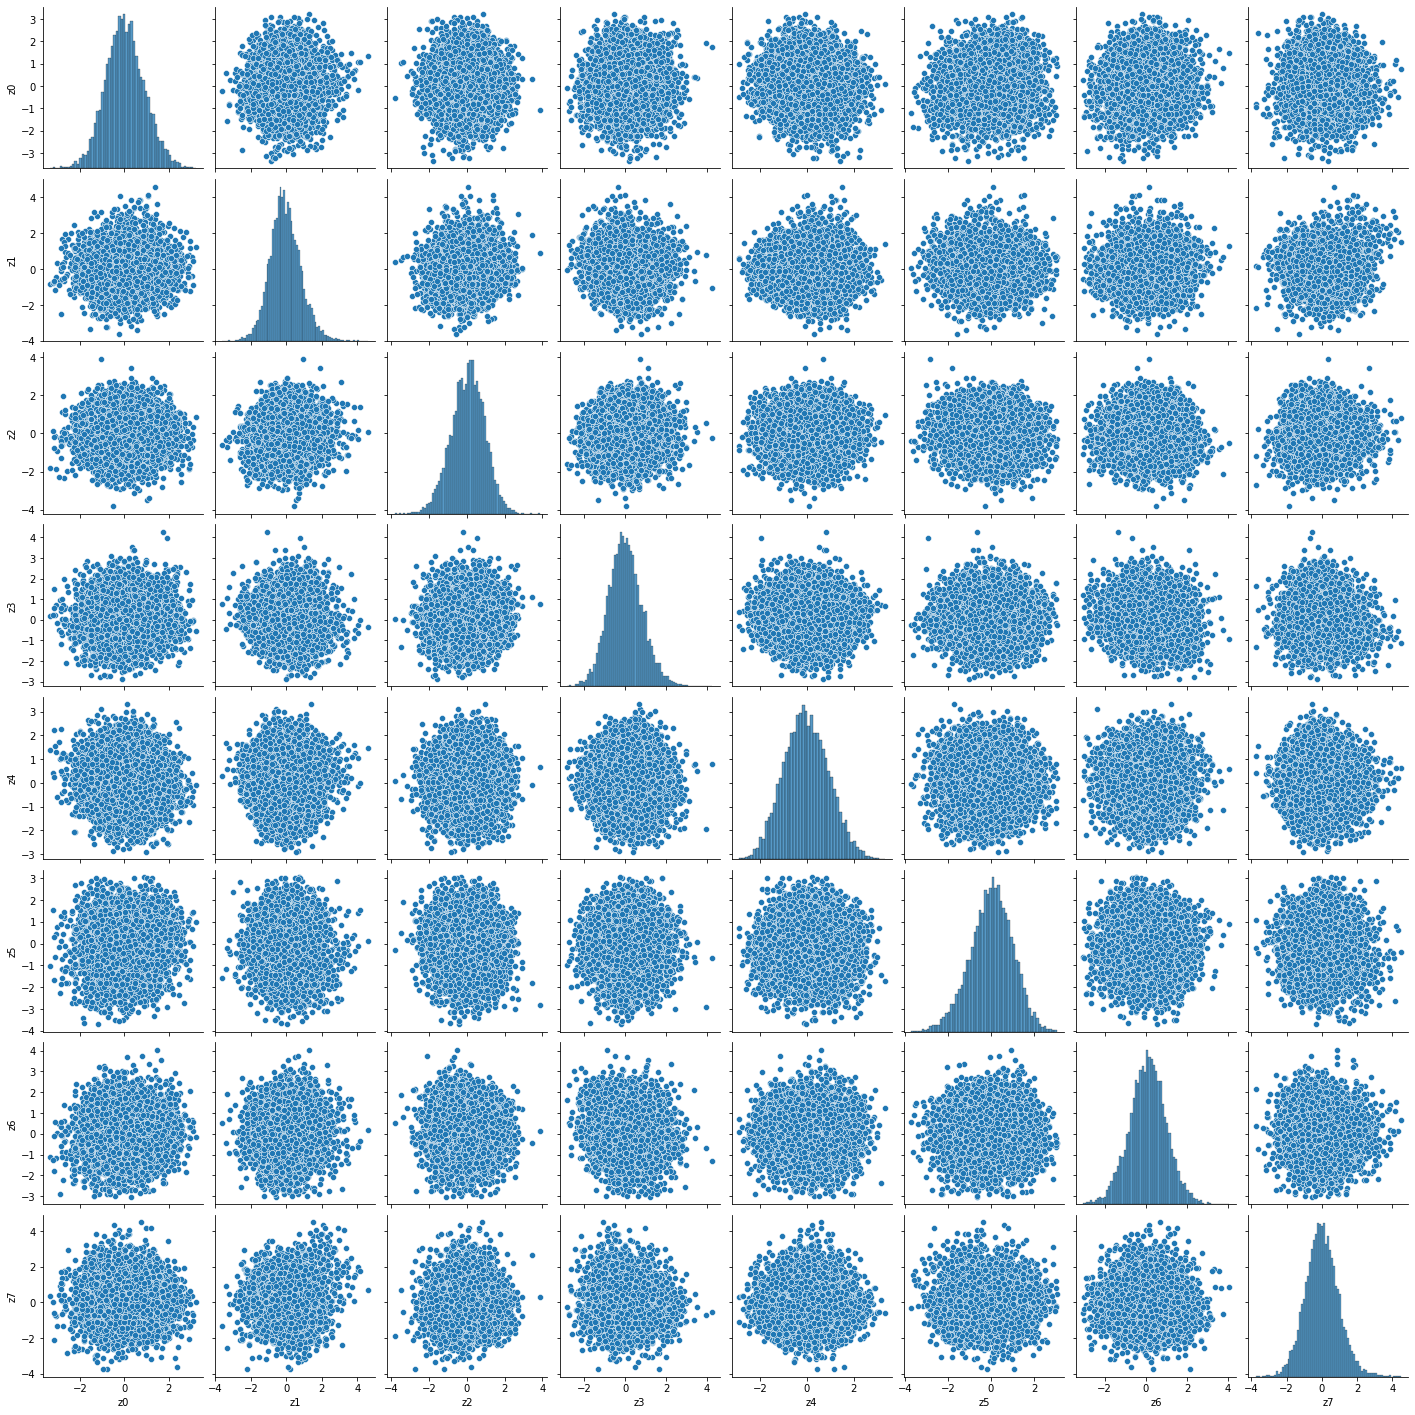
\includegraphics[width=\textwidth]{figs/supplementary/z_distribution.png}
 \caption{Distribution of the 8 latent variables for the experiment on unscaled meshes whose results are presented in the main text.}
 \label{fig:z_distribution}
\end{figure}

\subsubsection{Relation with health outcomes}
\textcolor{blue}{Check selection criteria of subjects who undergo CMR imaging.}

\textcolor{blue}{UK Biobank individuals with CMR images who have cardiac pathologies are scarce in number due to the selection criteria for individuals who undergo CMR imaging.}

\subsection{GWAS}

In this section, we provide quantile-quantile plots, or Q-Q plots, for the GWAS that yielded significant associations. % For the readers' convenience, we explain how to interpret these plots in the following paragraph. 

% A Q-Q plot is simply a way to compare two frequency distributions, $p_1$ and $p_2$, where $\int p_i(x)dx=1$. If $p_1$ and $p_2$ are continuous distributions, the associated Q-Q plot is built by matching the values that correspond to the same quantiles en each distribution, i.e. the graph is given by $\{(x,y): \int_{-\infty}^xp_1(t)dt=\int_{-\infty}^yp_2(t')dt'\}$
% In this case, it is employed to compare the distribution of $-\log_{10}(p)$ obtained by the GWAS and the same distribution if the $p$-values were uniformly distributed in $[0,1]$, which would be the case if the null hypothesis were true for all the tests. If there is some genetic signal present (i.e. the null hypothesis is rejected for some SNPs), then one should expect a deviation from the identity line. In summary, Q-Q plots provide a convenient way to easily tell whether a GWAS has yielded any significant association.

Figures \ref{fig:qq_scaled} and \ref{fig:qq_unscaled} show the Q-Q plots for the GWAS performed on the latent representations of scaled and unscaled meshes, respectively.

\begin{figure}
 \centering
 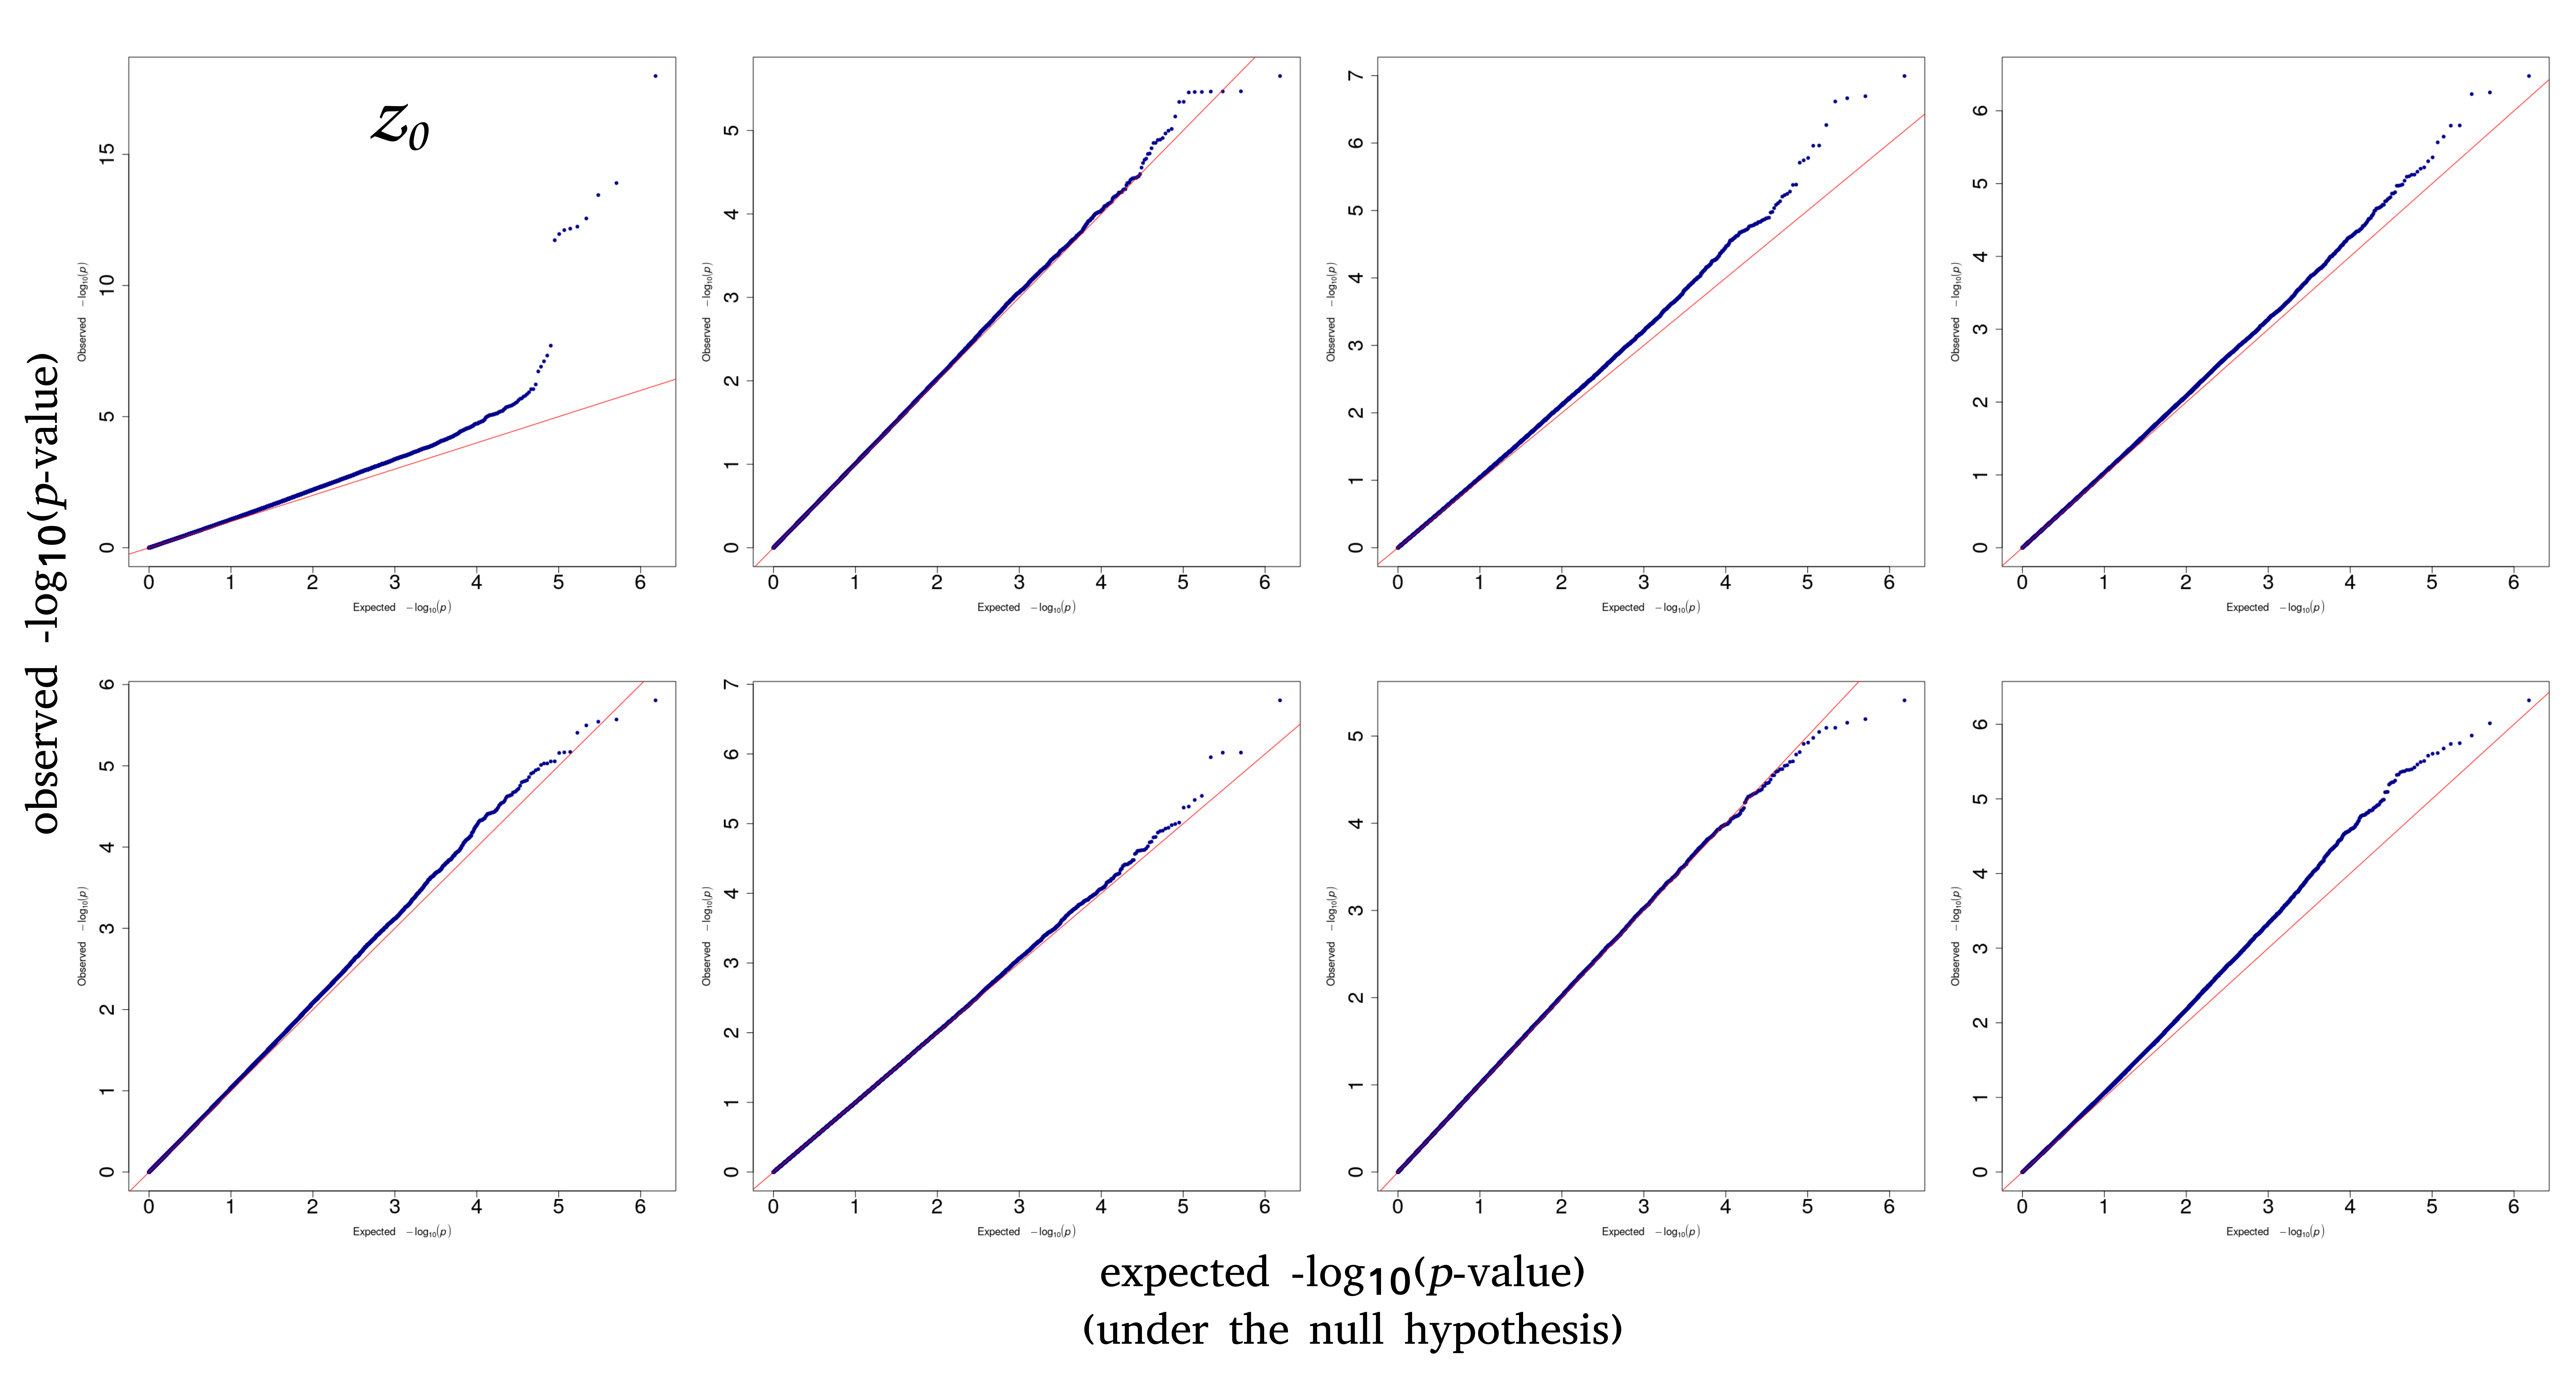
\includegraphics[width=\textwidth]{figs/supplementary/scaled_qq.png}
 \caption{Q-Q plots for the GWAS on each of the 8 latent variables of scaled LV meshes. Latent variable $z_0$, presented in the main text, is the only one showing a significant association.}
 \label{fig:qq_scaled}
\end{figure}

\begin{figure}
 \centering
 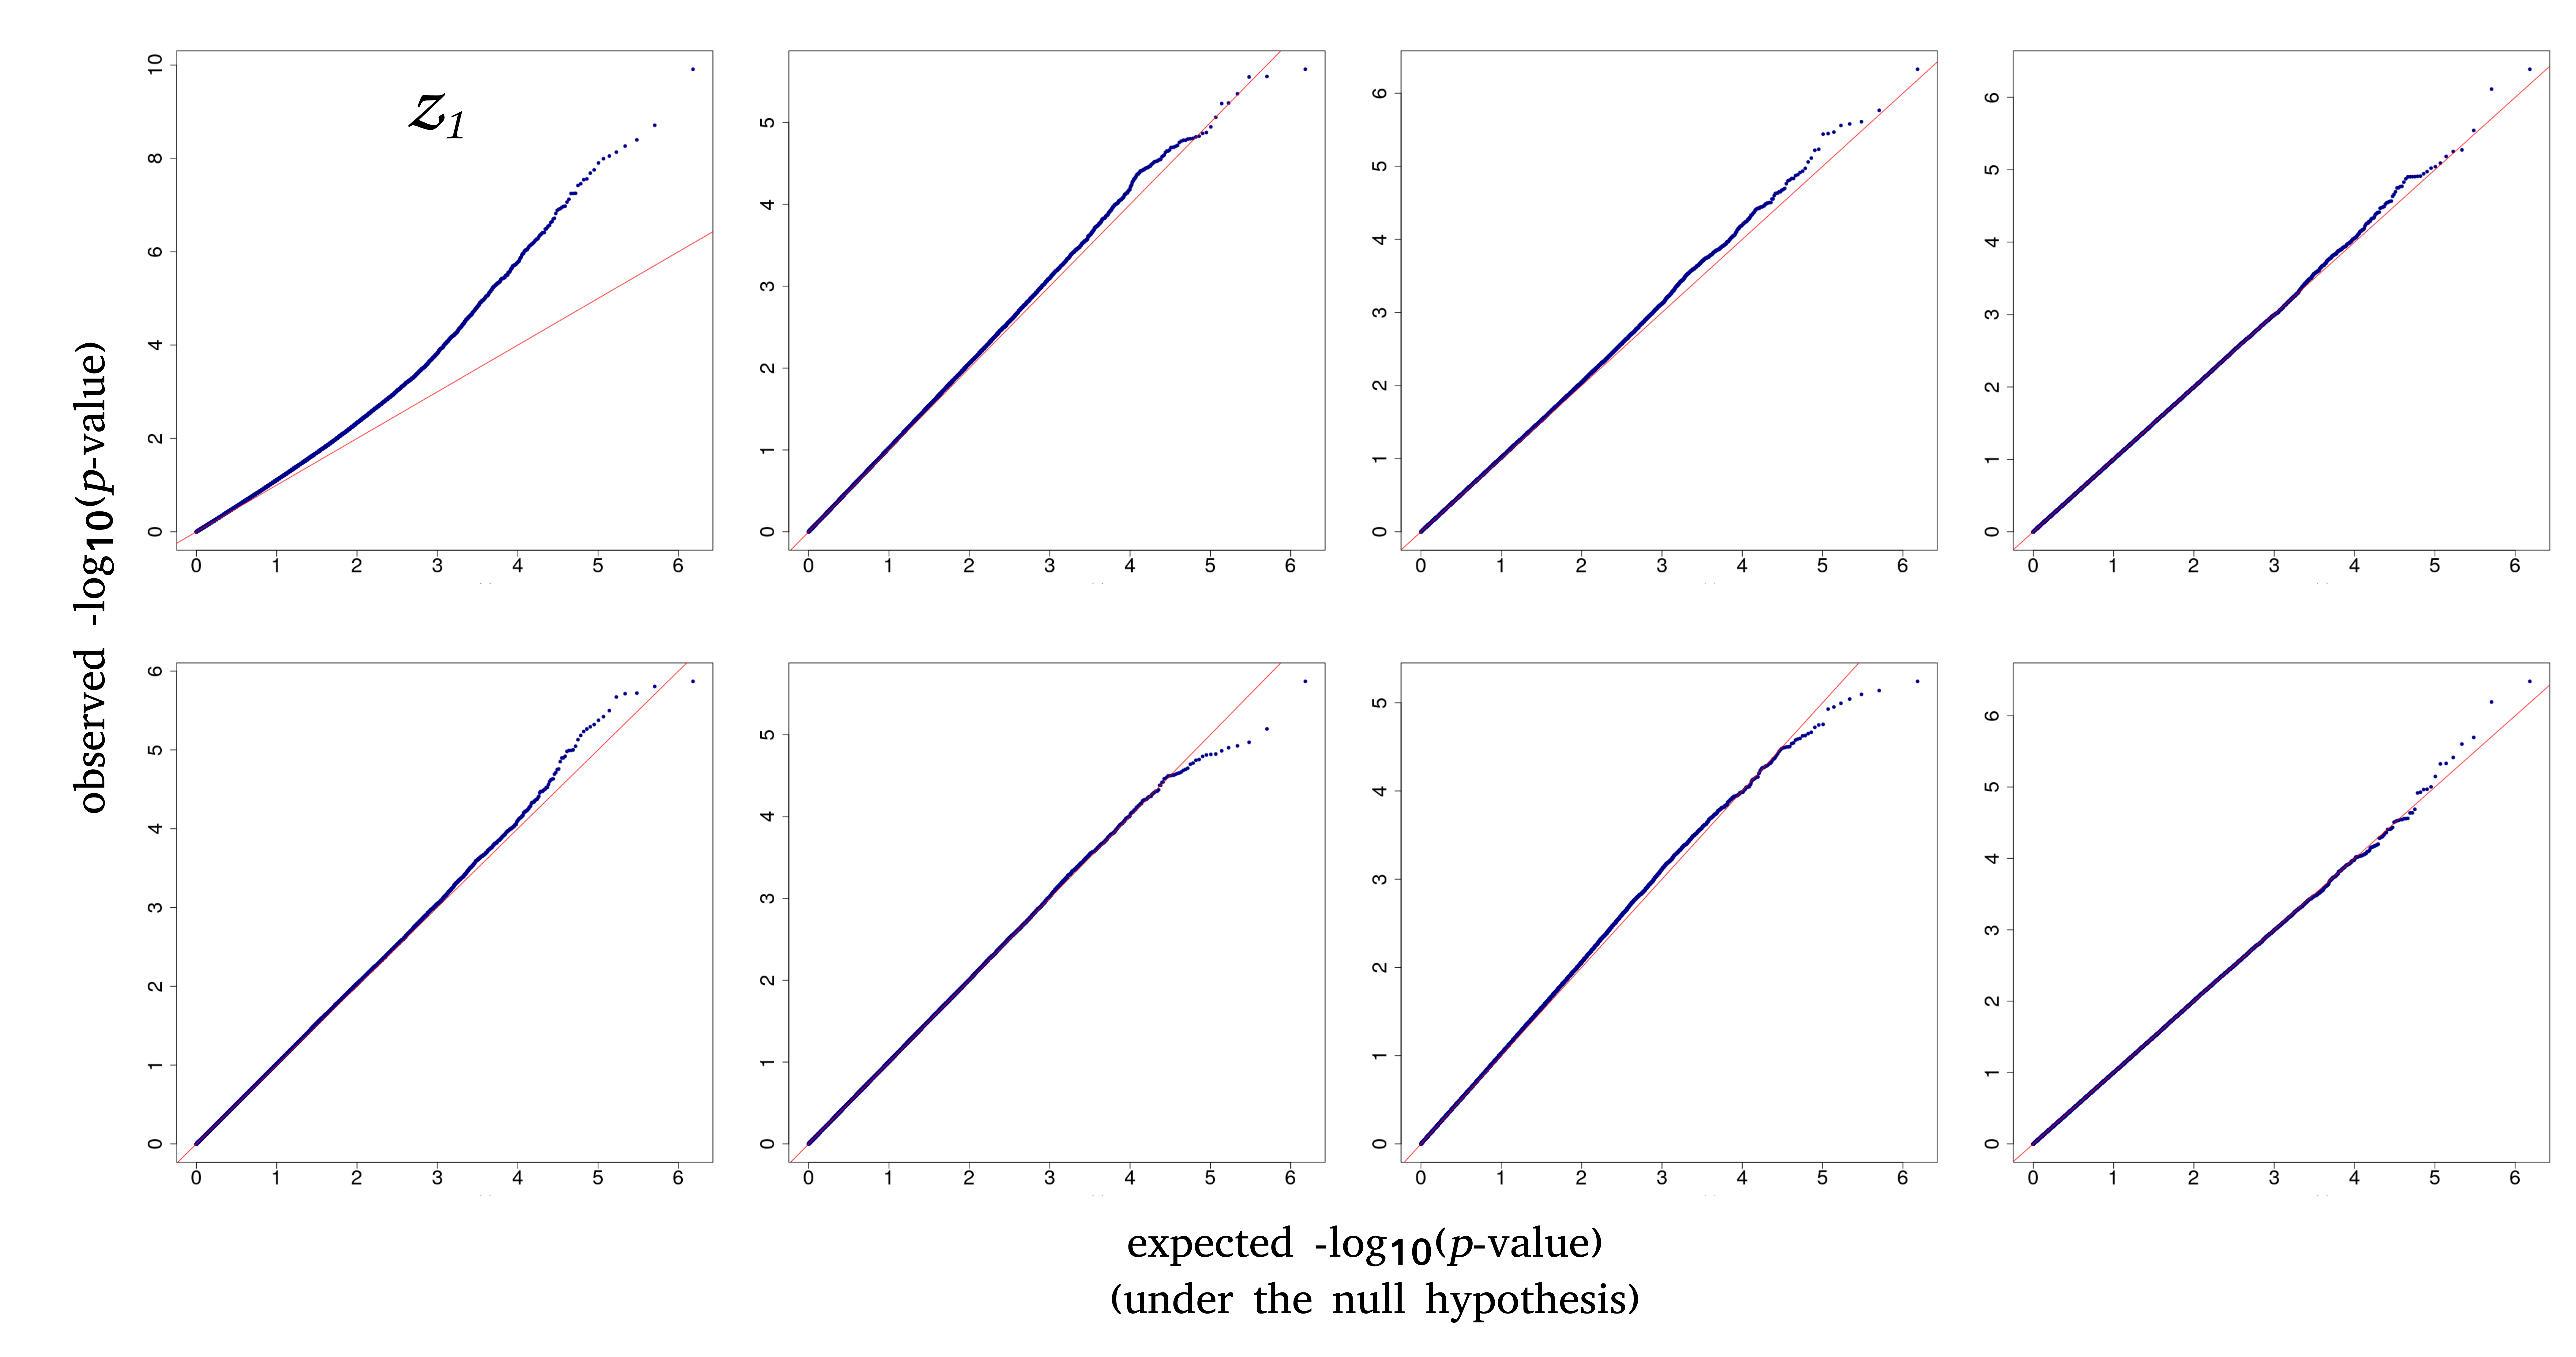
\includegraphics[width=\textwidth]{figs/supplementary/unscaled_qq.png}
 \caption{Q-Q plots for the GWAS on each of the 8 latent variables of unscaled LV meshes (i.e. meshes preserving the original scale from the images). Latent variable $z_1$, presented in the main text, is the only one showing significant associations.}
 \label{fig:qq_unscaled}
\end{figure}

\end{document}